\documentclass{ximera}


\author{Anna Davis} \title{MTH 140 Final Exam} 

\begin{document}

\begin{abstract}

\end{abstract}
\maketitle
 \textit{You have 1 hour and 50 minutes to complete this test.  Each answer is worth 1 point.}
\begin{problem}\label{prob:140finalprob1}
A fair coin is tossed Twice.  
\begin{enumerate}
    \item Fill out the following table to help you determine probabilities of obtaining various outcomes.
    
\begin{center}
\begin{tabular}{|c|c|c|}
 \hline
 &&   \\
 & H& T  \\
 &&   \\
  \hline
  &&\\
 H&$\answer{HH}$&$\answer{HT}$ \\
  && \\
 \hline
  &&\\
 T&$\answer{TH}$&$\answer{TT}$ \\
  && \\
 \hline
 \end{tabular}
\end{center}    
\item Probability of getting one tail: $\answer{0.5}$

\item Probability of getting two heads: $\answer{\frac{1}{4}}$
\item Probability of getting three tails: $\answer{0}$
\end{enumerate}
\end{problem}

\begin{problem}\label{prob:140finalprob2}
A real estate agent finds the following regression line for predicting the price of a house ($y$), in thousands of dollars, from the square footage ($x$).

$$y = 160.2 + 0.09x$$

Based on this model, the price of a 2,300 sq. foot house will be $\answer{367.2}$ thousand dollars.
\end{problem}

\begin{problem}\label{prob:140finalprob3}
Alice (A), Ben (B), Catherine (C) and Doug (D) took the same biology test.  Their results are listed below: 

Alice's score is in the $90$th percentile 

Ben's $z$-score is $z = 2$ 

Catherine's score is in the $10$th percentile 

Doug's $z$-score is $z = 0$

Arrange students’ initials (A, B, C and D) in order of increasing test results (lowest test result to highest test result).  Enter your answer as a single string, all capitals, no spaces.  e.g. ABCD.
$$\answer[format=string]{CDAB}$$
\end{problem}

\begin{problem}\label{prob:140finalprob4}
A sample of size $40$ is drawn from a population whose standard deviation is $10.4$.  The sample mean is $74.5$.  Construct a 99\% confidence interval.

Summary of given info:
$$\sigma=\answer{10.4}$$
$$\overline{x}=\answer{74.5}$$
$$n=\answer{40}$$
Use the Critical $z$-value table to find $z_{\alpha/2}$
$$z_{\alpha/2}=\answer{2.575}$$
Error Bound for the Mean:
$$EBM=\answer{2.575}\frac{\answer{10.4}}{\answer[tolerance=0.01]{\sqrt{40}}}=\answer[tolerance=0.01]{4.2343}$$
The 99\% confidence interval is:
$$(\answer[tolerance=0.1]{70.27},\answer[tolerance=0.1]{78.73})$$
\end{problem}

\begin{problem}\label{prob:140finalprob5}
Use the screenshot below to answer the questions.  

\begin{center}
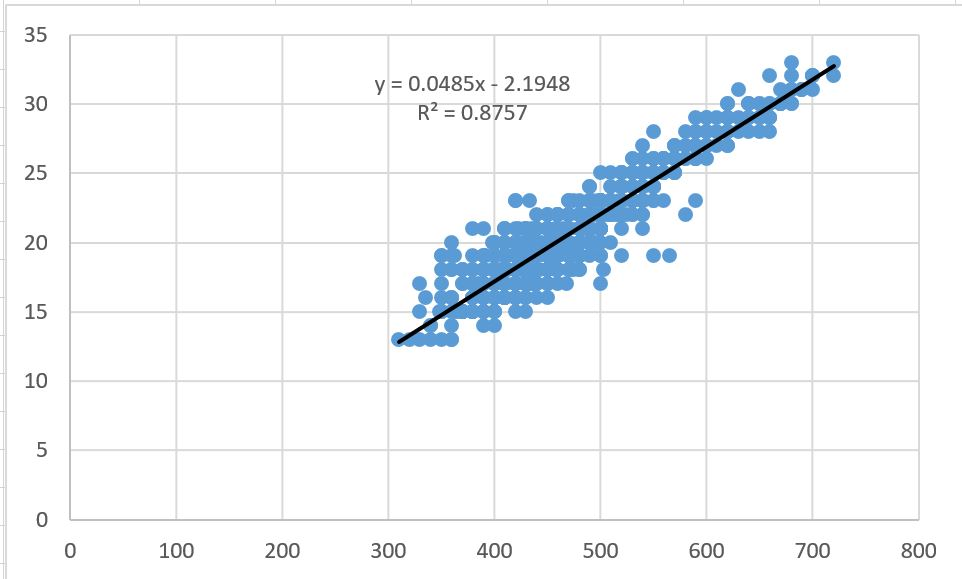
\includegraphics[height=2in]{140finalpic1.jpg}
\end{center}

Compute the correlation coefficient $r$.
 $$r=\answer[tolerance=0.01]{0.9378}$$
\end{problem}

\begin{problem}\label{prob:140finalprob6}
Use the table below to compute sample standard deviation, ($s$), for the following SAMPLE of test scores:
$$68, 73, 75, 81, 94$$

$$\overline{x}=\answer{78.2}$$
Enter EXACT values into the table; no rounding.
\begin{center}
\begin{tabular}{|c|c|c|}
Test Scores & Deviations & Deviations Squared  \\
 \hline
 \hline
   & &\\
 68 &$\answer{-10.2}$  & $\answer{104.04}$ \\
  & &\\
  \hline
   & &\\
 73 &$\answer{-5.2}$  & $\answer{27.04}$\\
  & &\\
 \hline
  & &\\
 75 &$\answer{-3.2}$ &$\answer{10.24}$ \\
  & &\\
 \hline
  & &\\
 81 &$\answer{2.8}$  &$\answer{7.84}$ \\
  & &\\
 \hline
  & &\\
 94 &$\answer{15.8}$  &$\answer{249.64}$ \\
  & &\\
 \hline
  
\end{tabular}
\end{center}
$$s =\sqrt{\frac{\sum (x-\overline{x})^2}{n-1}}=\answer[tolerance=0.1]{10}$$
\end{problem}

\begin{problem}\label{prob:140finalprob7}
Find mean, median, Q1 and Q3 for the following data. 
$$11, 14, 9, 17, 19, 22, 8, 12, 20, 24$$

Mean:  $\mu=\answer{15.6}$

Median:  $M=\answer{15.5}$

$Q1=\answer{11}$

$Q3=\answer{20}$

$IQR=\answer{9}$
\end{problem}

\begin{problem}\label{prob:140finalprob8}
An ice-cream shop claims that one scoop of ice-cream is 50 grams.  You may assume that ice-cream amounts per scoop are normally distributed.  An inspector is wondering if the amount of ice-cream in one scoop is less than 50 grams.  He tests a random sample of 60 scoops.  The sample mean is found to be 49.2 grams, with sample standard deviation of 2.2 grams.  Conduct a hypothesis test to determine if the average amount of ice-cream in one scoop is less than 50 grams.  Use $\alpha=0.05$.

$$\overline{x}=\answer{49.2},\quad s=\answer{2.2},\quad n=\answer{60},\quad df=\answer{59}$$
Null Hypothesis
$$H_0:\quad \mu=\answer{50}$$
Alternative Hypothesis
$$H_a:\quad \mu<\answer{50}$$
Find the $t$-score (round to three decimal places)
$$t=\answer[tolerance=0.01]{-2.817}$$
Find the $p$-value
\begin{center}  
\geogebra{emwxhga2}{800}{600}  
\end{center}
$$p=\answer[tolerance=0.001]{0.0033}$$
Decision:

\begin{multipleChoice} 
\choice[correct]{$p$-value is less than 0.05.  We reject the null hypothesis.}  
\choice{$p$-value is less than 0.05.  We do not reject the null hypothesis.} 
\choice{$p$-value is greater than 0.05.  We reject the null hypothesis.} 
\choice{$p$-value is greater than 0.05.  We do not reject the null hypothesis.}  
\end{multipleChoice}  

Conclusion:

\begin{multipleChoice} 
\choice{At the 0.05 level of significance, we have proved the null hypothesis.}  
\choice{At the 0.05 level of significance, there is not enough evidence to make any conclusions.} 
\choice[correct]{At the 0.05 level of significance, there is enough evidence to conclude that the mean amount of ice-cream per scoop is less than 50 grams.}  
\choice{At the 0.05 level of significance, there is not enough evidence to conclude that the mean amount of ice-cream per scoop is less than 50 grams.} 
\end{multipleChoice} 
\end{problem}

\begin{problem}\label{prob:140finalprob9}
The data for the height of women is approximately bell-shaped.  If a woman’s height has a z-score of -0.52, what percentage of women is shorter than she is?

Approximately $\answer[tolerance=0.1]{30.15}$\% of women are shorter.
\end{problem}

\begin{problem}\label{prob:140finalprob10}
Suppose exam scores on the first Chemistry test at a large university are normally distributed with a mean of 71 and standard deviation of 10.5. What percentage of students scored above 80?

Approximately $\answer[tolerance=0.1]{19.6}$\% of students scored above 80.
\end{problem}


\end{document} 